Over the years, Google has been building its own distinctively designed data
centers, deploying numerous machines around the world. Within these facilities,
arrays of servers operate continuously, fueling essential services that a
multitude of people rely on daily. Nevertheless, the process of designing data
centers is a complex optimization challenge with multiple factors to consider.
While the primary objective is to optimize the utilization of computing capacity
offered to users, it is equally imperative to ensure the uninterrupted provision
of computing power, even in scenarios where hardware failures are inevitable.
Based on this motivation, Google invites participants to address these
challenges in a (fictional) Google Data Center modelled after a real-world
scenario, which we described next.

The data center, as outlined in the problem statement, is modelled as set of
distinct~\textit{rows}, each comprising a certain number of available spaces
known as~\textit{slots}, where servers can be positioned. It is worth
highlighting that rows share resources, including electric power, Consequently,
in the event of a hardware failure, an entire row of servers may become
inaccessible, impacting the entirety of the servers located within that row.
Moreover, the maximum number of slots is consistent across all rows within the
data center. However, not all slots may be accessible due to specific
installations or requirements that impose restrictions on the use of certain
spaces.

In ~\Cref{fig:data-center-layout}, an illustration depicts a layout
featuring two rows, each consisting of a total of seven slots. Some of these
slots are marked as unavailable as indicated by the cross symbol.

\begin{figure}[h]
  \centering
  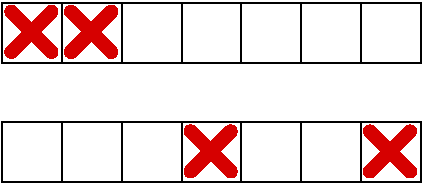
\includegraphics[width=0.6\textwidth,keepaspectratio]{../assets/dc/dc-rows-no-labels.pdf}
  \caption{Example Data Center Layout}
  \label{fig:data-center-layout}
\end{figure}

The servers are defined by a tuple that includes two attributes: the
\textit{size} of the server, which is measured in terms of the number of
consecutive slots occupied by the machine, and the computing~\textit{capacity}
of the server, represented as an integer value that indicates the machine's CPU
resources.~The~\Cref{table:dc-example-properties} presents potential values for
these parameters, showcasing examples of four distinct servers.

\begin{table}[ht]
  \centering
  \begin{tabular}{ccc}
  \toprule Server & Size &
  Capacity                    \\ \midrule
  1               & 3    & 2  \\
  2               & 2    & 5  \\
  3               & 3    & 10 \\
  4               & 2    & 3  \\
  \bottomrule
\end{tabular}
  \caption{Server Properties}
  \label{table:dc-example-properties}
\end{table}

Moreover, when servers are positioned within the data center rows, they are
logically associated with resource~\textit{pools}, to which they can contribute
their individual computing capacities.~The capacity of a pool is defined as the
collective sum of the capacities of all the servers allocated to it.

For clarification,~\Cref{fig:data-center-layout-with-servers} offers a potential
assignment of servers based on the data center layout depicted in
~\Cref{fig:data-center-layout}, and the server attributes provided
in~\Cref{table:dc-example-properties}. In this particular case, servers are
allocated to two distinct resource pools.

\begin{figure}[h]
  \centering
  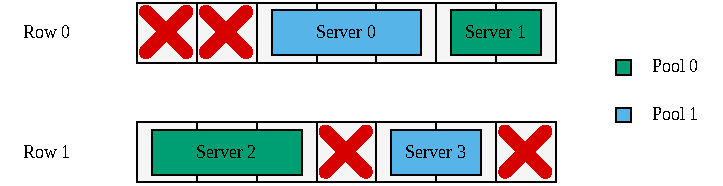
\includegraphics[width=0.9\textwidth,keepaspectratio]{../assets/dc/dc-example.pdf}
  \caption{Example Server Assignment}
  \label{fig:data-center-layout-with-servers}
\end{figure}

Upon closer examination of the this example, we can deduce that ensuring the
reliability of a specific resource pool implies the distribution of servers
across various rows. This approach ensures that in the event of a row failure,
the pool can still operate with diminished capacity, drawing upon the servers
located in the unaffected rows.~In the context of the problem, this represents
the concept of a~\textit{guaranteed capacity} for a pool, which can be defined
as follows:

Given a resource pool ($p$), the guaranteed capacity of that ($gc_{p}$) is a
measure of the remaining computing capacity available in the event that at most
one arbitrary row~($r \in \mathcal{R}$) of the data center becomes unavailable.
Formally, this can be described as shown in~\Cref{eq:guaranteed-capacity}, where
$\mathcal{M}$ denotes the set of servers (machines) available and $c_{m}$ the
computing capacity of a given server ($m \in \mathcal{M}$).

\begin{equation}
  \label{eq:guaranteed-capacity}
  {gc}_{p} = \min_{r \in \mathcal{R}} \left({\sum_{m \in \mathcal{M} \land m \in p} c_{m}} - {\sum_{ m \in \mathcal{M} \land m \in p \land m \in r} c_{m}}\right)
\end{equation}

In essence, the objective of this problem can be succinctly defined as:
Given a layout description of a data center, the objective is to determine the
optimal arrangement of servers within the data center rows and assign these
servers to resource pools, such that, the minimum guaranteed capacity across all
pools is maximized. Mathematically, this can be expressed as shown in Equation
\ref{eq:objective}, where $s$ represents a candidate solution, $\mathcal{P}$
the set of pools, and $gc_{p}$ denotes the guaranteed capacity for a specific
pool ($p \in \mathcal{P}$).

\begin{equation}
  \label{eq:objective}
  \max f(s) = \min_{p \in \mathcal{P}} \left({gc}_{p}\right)
\end{equation}

Moreover, in a competition context, the value obtained from evaluating a
solution represents the score a contestant would attain for solving a particular
instance of this problem. For clarification of all the aforementioned concepts,
the~\Cref{ex:problem-scoring} illustrates the scoring process of a candidate
solution.

\begin{example}[Scoring]
  \label{ex:problem-scoring}
  Regarding the data center layout shown
  in~\Cref{fig:data-center-layout-with-servers} and the server properties
  provided in~\Cref{table:dc-example-properties}, we can summarize
  the capacities assigned to each resource pool, by row, as shown in~\Cref{table:dc-gc-example}.

  \begin{table}[ht]
    \centering
    \begin{tabular}{@{\extracolsep{4pt}}cccccc@{\extracolsep{4pt}}}
  \toprule
  Pool & Row 1 & Row 2 & Guaranteed Capacity & \textbf{$f(x)$}              \\ \midrule
  1    & 5     & 10    & 5                   &                              \\
  2    & 2     & 3     & 2                   & \multirow{-2}{*}{\textbf{2}} \\
  \bottomrule
\end{tabular}
    \caption{Guaranteed Capacity \& Score}
    \label{table:dc-gc-example}
  \end{table}

  The score obtained for this server placement, as determined by the evaluation
  of the objective~\ref{eq:objective}, can thus be calculated as $\min(5, 2) = 2$.
\end{example}

Regarding the problem instances to be optimized, crucial details are provided
concerning the layout of the data center, the available servers for allocation,
and specifics about the unavailable slots.~These aspects are represented using
the following parameters and their corresponding constraints:

\begin{description}
  \item[\textbf{$\mathcal{R}$.}] ($ 1 \leq \mathcal{R} \leq 1000$) The number of rows in the data center.
  \item[\textbf{$\mathcal{S}$.}] ($ 1 \leq \mathcal{S} \leq 1000$) The number of slots in each row of the data center.
  \item[\textbf{$\mathcal{U}$.}] ($ 0 \leq \mathcal{U} \leq \mathcal{R} \times \mathcal{S}$) The number of unavailable slots.
  \item[\textbf{$\mathcal{P}$.}] ($ 1 \leq \mathcal{P} \leq 1000$) The number of resource pools.
  \item[\textbf{$\mathcal{M}$.}] ($ 1 \leq \mathcal{M} \leq \mathcal{R} \times \mathcal{S}$) The number of servers to be allocated.
\end{description}

Notably, in a compettion setting, participants were required to read and output
both the problem description details presented, and the solution obtained, in a specific
format as outlined in the problem statement. For a description of the these and
other considerations regarding mostly implementation and evaluation details, the
reader can refer to the official problem statement which can be found on the
Google Coding Competitions Archive~\cite{googlellc2023codingcompetitionsarchive}.

% This requirement can influence the practical representation
% of solutions and may impact the way the model is defined. However, from a
% conceptual standpoint, the representation itself is not of utmost importance, as
% it should be feasible to translate between different representations without
% losing any essential information. Therefore, while modeling the problem using
% the adopted modelling framework's proposed aspects, we used the representation
% that we found to be the most well-suited and efficient from an implementation
% standpoint, as opposed to the most convenient to work with.